\section{Results}
\label{sec:results}

\subsection{Hidden States Encode Failure Risk}
\label{sec:safety_encoding}

\begin{figure}[t]
    \centering
    \begin{subfigure}[t]{0.47\linewidth}
        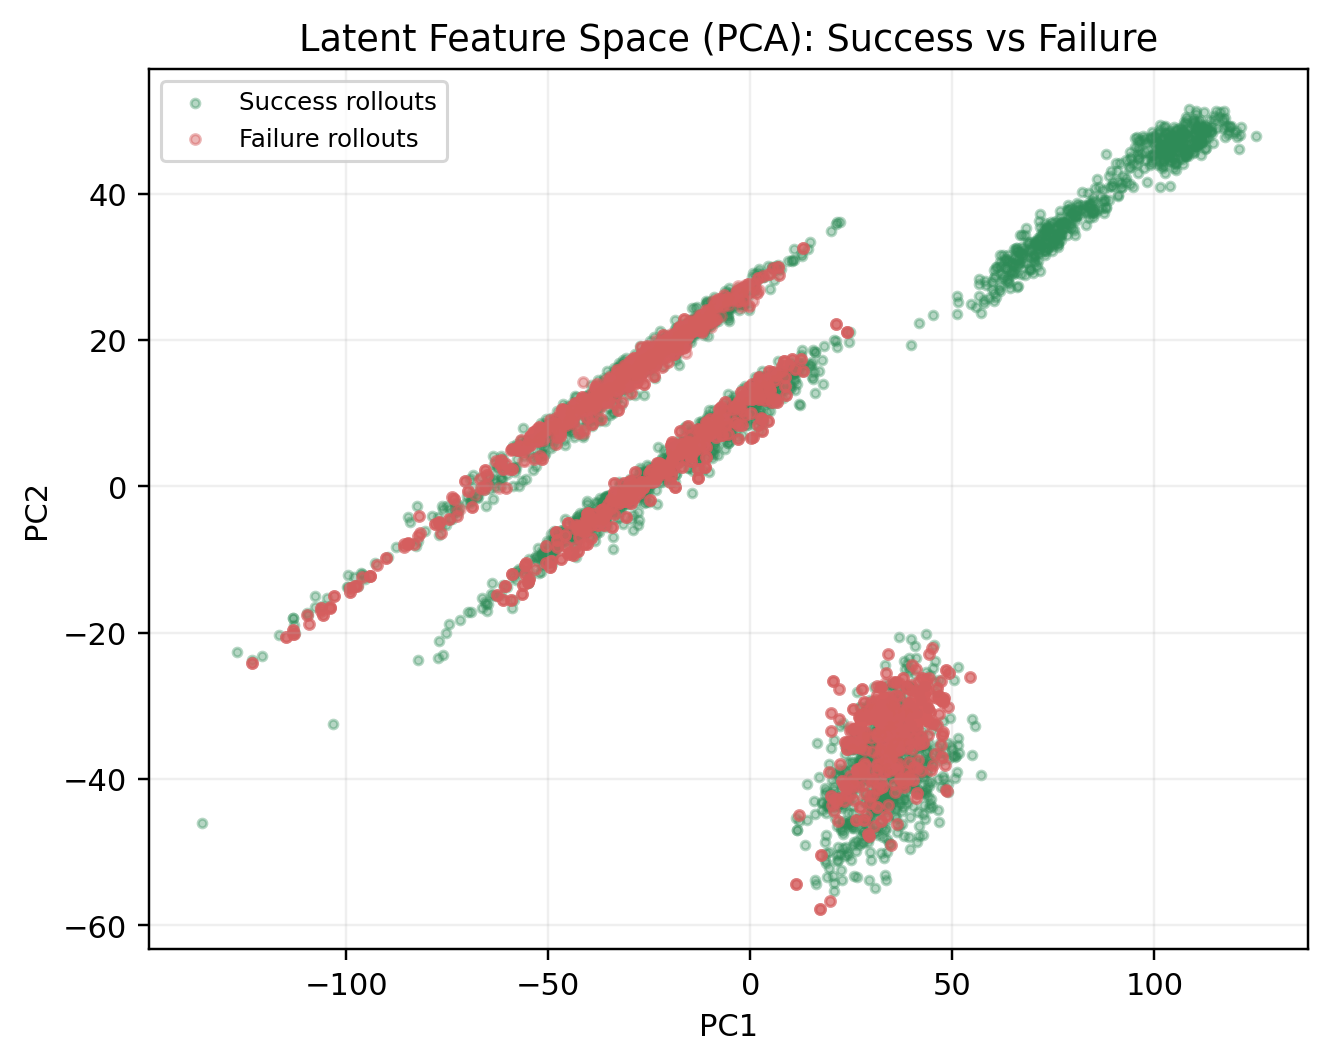
\includegraphics[width=\linewidth]{figures/17_latent_pca_success_failure.png}
        \caption{PCA of OpenVLA hidden states. Success and failure separate along the first two principal components.}
        \label{fig:latent_pca}
    \end{subfigure}
    \hfill
    \begin{subfigure}[t]{0.47\linewidth}
        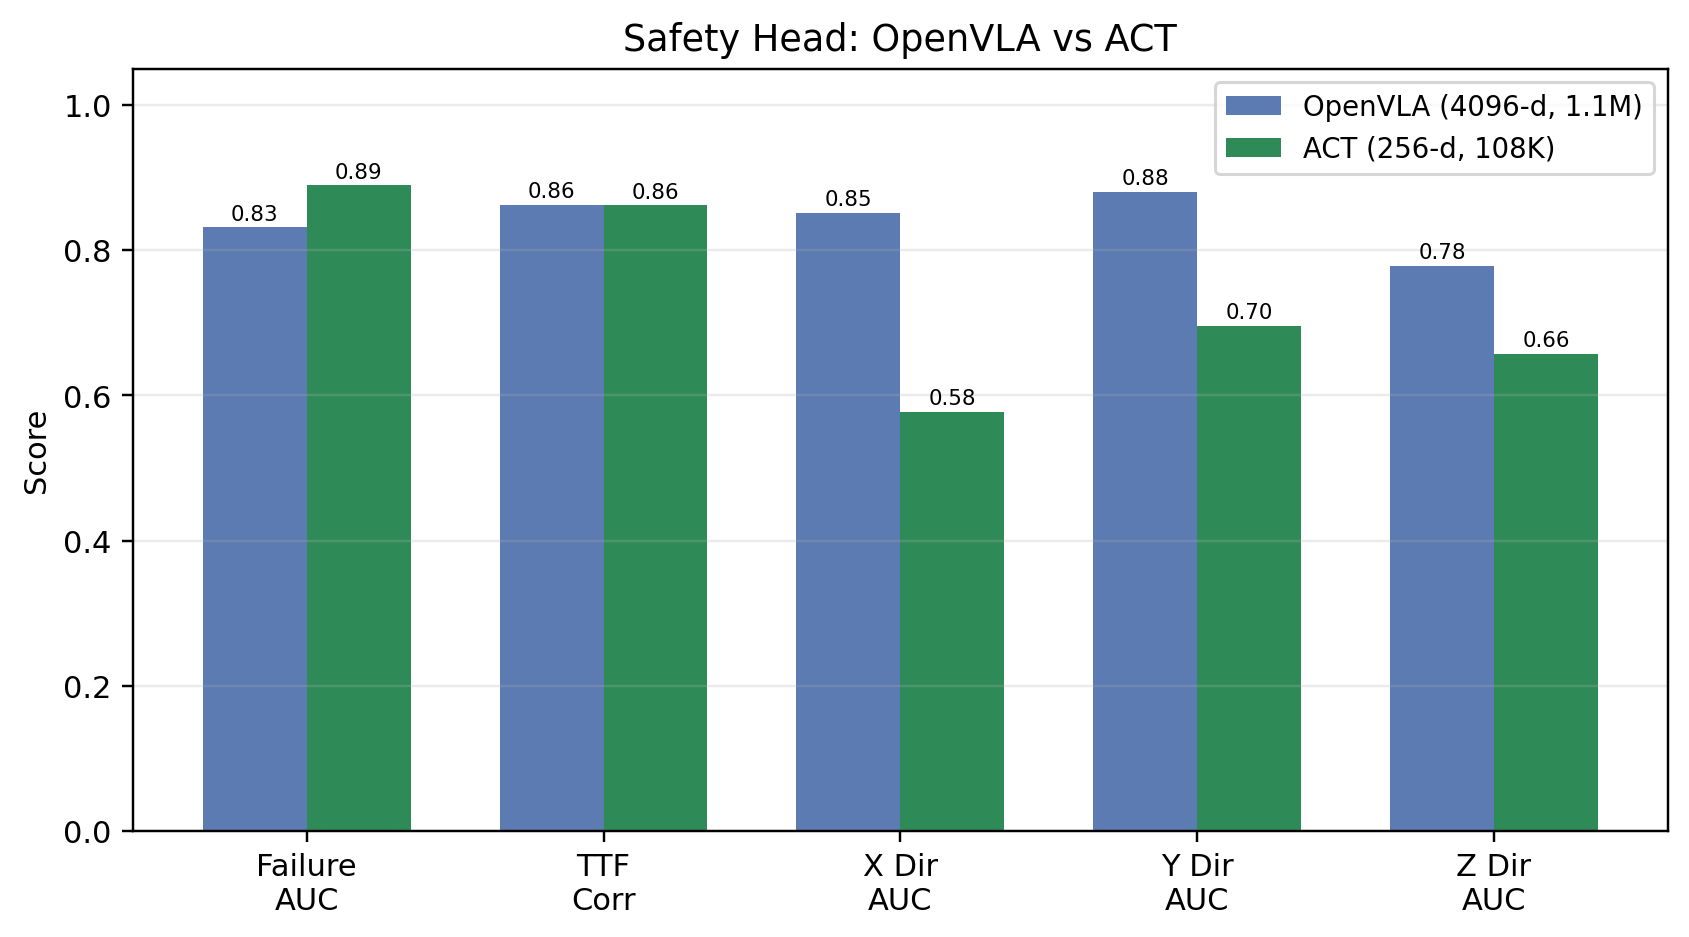
\includegraphics[width=\linewidth]{figures/24_safety_head_auc.png}
        \caption{Probe AUC across architectures. Failure detection is strong on both; correction AUC is weaker on ACT, foreshadowing \S\ref{sec:mechanism}.}
        \label{fig:safety_head_auc}
    \end{subfigure}
    \caption{\textbf{Failure risk is nonlinearly encoded in hidden states.} The MLP probe gains $+0.05$/$+0.10$ AUC over a linear baseline on OpenVLA/ACT despite a $16{\times}$ feature-dimensionality gap.}
    \label{fig:encoding}
\end{figure}

\begin{table}[t]
\centering
\caption{Safety head metrics on the trajectory-disjoint held-out test set. \emph{Chance} is random guessing; \emph{linear probe} is L2-regularized logistic regression on the same hidden states and split, isolating linearly accessible failure signal. \textbf{PULSE} is the trained MLP probe. The correction-head AUCs are kept for reference; the mechanism analysis (Section~\ref{sec:mechanism}) shows the correction direction does not outperform random perturbation despite the apparent gap over chance. \emph{Provenance:} Failure AUCs are read from \texttt{hpc\_mirror/checkpoints/eef\_correction\_mlp/results.json} (and the ACT analog), produced by \texttt{scripts/train\_eef\_correction\_mlp.py} on the OpenVLA-seed0 / ACT-spatial rollout pools with a 75/15/10 rollout-level split (\texttt{np.random.shuffle} under \texttt{np.random.seed}). The post-hoc threshold-replay AUCs reported in Table~\ref{tab:threshold_operating} are slightly higher because they use a larger merged rollout pool and a different RNG (see Appendix~\ref{app:auc_reconciliation}).}
\label{tab:safety_head_metrics}
\begin{tabular}{lcc}
\toprule
Metric & OpenVLA (4096-d) & ACT (256-d) \\
\midrule
\textit{Failure AUC --- chance} & 0.500 & 0.500 \\
\textit{Failure AUC --- linear probe baseline} & 0.785 & 0.788 \\
\textbf{Failure AUC --- PULSE (ours)} & \textbf{0.832} & \textbf{0.889} \\
$\Delta$ AUC over linear baseline & $+0.047$ & $+0.101$ \\
\midrule[0.4pt] Failure Accuracy ($\sigma{\geq}0.5$) & 0.773 & 0.793 \\
\midrule[0.4pt] \textit{TTF correlation --- chance} & 0.000 & 0.000 \\
\textbf{TTF Correlation ($r$) --- PULSE (ours)} & \textbf{0.863} & \textbf{0.862} \\
TTF $R^2$ & 0.741 & 0.739 \\
\midrule[0.4pt] \textit{Correction cosine --- chance (random unit)} & 0.000 & 0.000 \\
Correction Cosine Sim (median) & 0.794 & 0.565 \\
\textit{X Direction AUC --- chance} & 0.500 & 0.500 \\
X Direction AUC & 0.851 & 0.578 \\
\textit{Y Direction AUC --- chance} & 0.500 & 0.500 \\
Y Direction AUC & 0.880 & 0.696 \\
\textit{Z Direction AUC --- chance} & 0.500 & 0.500 \\
Z Direction AUC & 0.779 & 0.657 \\
\midrule[0.4pt] Parameters & 1,099,397 & 108,677 \\
\bottomrule
\end{tabular}
\end{table}


\begin{figure}[t]
    \centering
    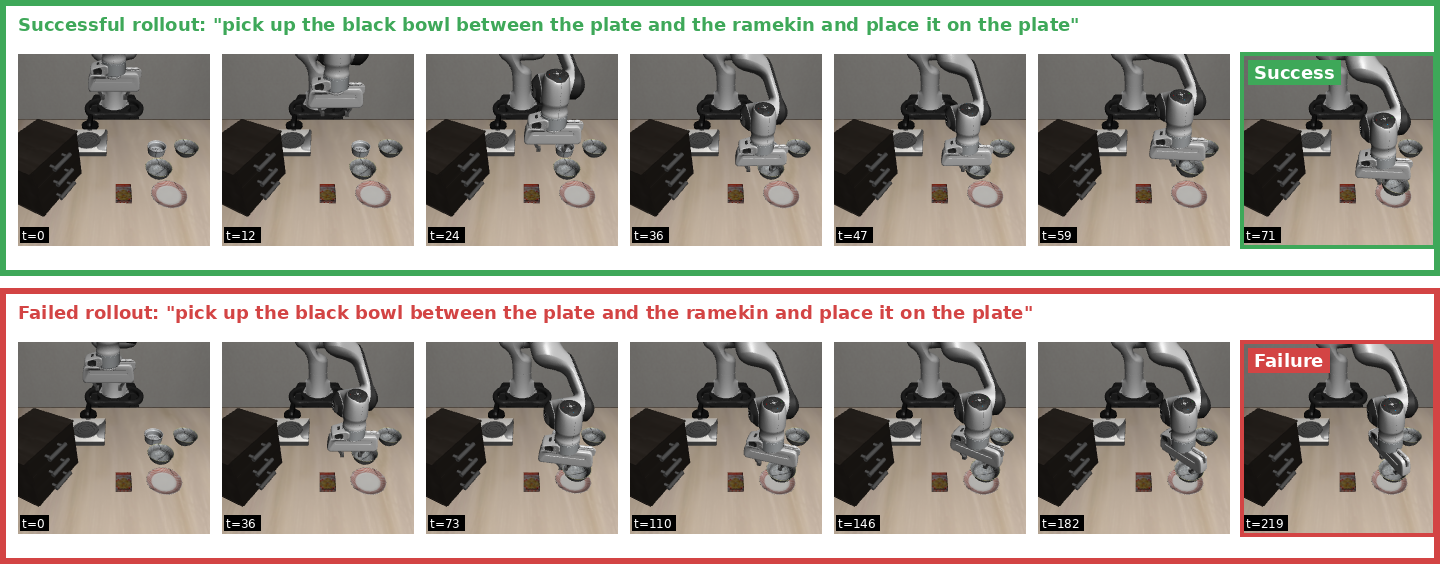
\includegraphics[width=\linewidth]{figures/28_success_failure_rollout.png}
    \caption{\textbf{Success (green) vs.\ failure (red) rollout filmstrips} on LIBERO-Spatial Task~0. Each row is a recorded policy rollout replayed from its own logged simulator state. The success row picks the \texttt{akita\_black\_bowl} and places it on \texttt{plate\_1}; the failure row approaches the bowls but does not complete the placement.}
    \label{fig:rollout_filmstrip}
\end{figure}

MLP probes trained on frozen hidden states achieve failure-detection AUC $0.83$ (OpenVLA) and $0.89$ (ACT), gaining $+0.05$/$+0.10$ over a linear-probe baseline (Table~\ref{tab:safety_head_metrics}, Fig.~\ref{fig:encoding}). The same probe template trains from scratch on both architectures with no modification, despite the $16{\times}$ dimensionality gap. The TTF head reaches $r{=}0.86$ on both; on LIBERO-Spatial, a raw step-counter baseline matches PULSE on TTF (Appendix~\ref{app:temporal_baseline})---failure rollouts run to a fixed 300-step length---so the clock-free contribution is the failure-detection AUC. Correction-head AUCs (0.78--0.88 on OpenVLA; 0.58--0.70 on ACT) foreshadow the mechanism result in \S\ref{sec:mechanism}.

\subsection{Inference Optimization: Single-Step Gating Matches $K$-Sample Search at $6.1\times$ Lower Latency}
\label{sec:steering_results}

\begin{figure}[t]
    \centering
    \begin{subfigure}[t]{0.47\linewidth}
        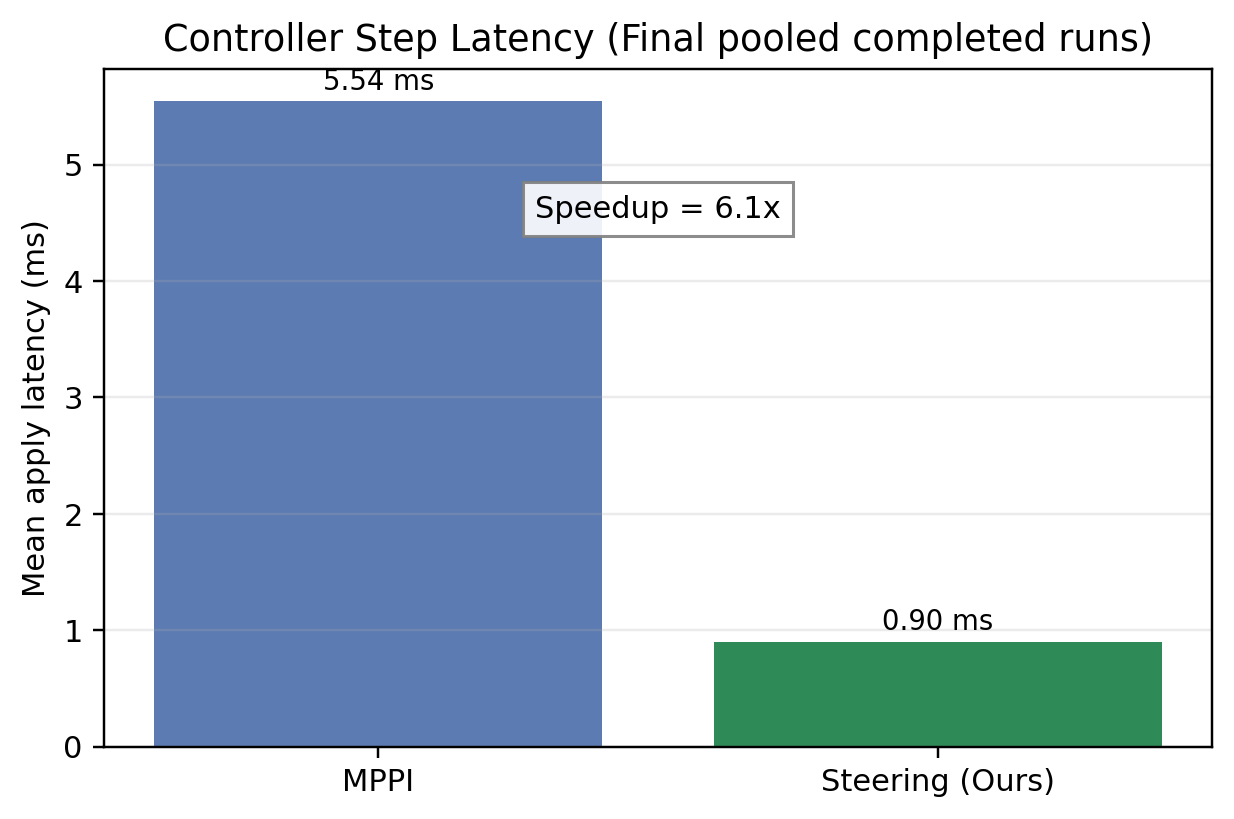
\includegraphics[width=\linewidth]{figures/09_latency_speedup_ood.png}
        \caption{Per-step apply time: single-step gating ($0.9$\,ms) vs.\ K-sample MPPI ($5.6$\,ms). Speedup holds across OOD disturbance levels.}
        \label{fig:latency_bar}
    \end{subfigure}
    \hfill
    \begin{subfigure}[t]{0.47\linewidth}
        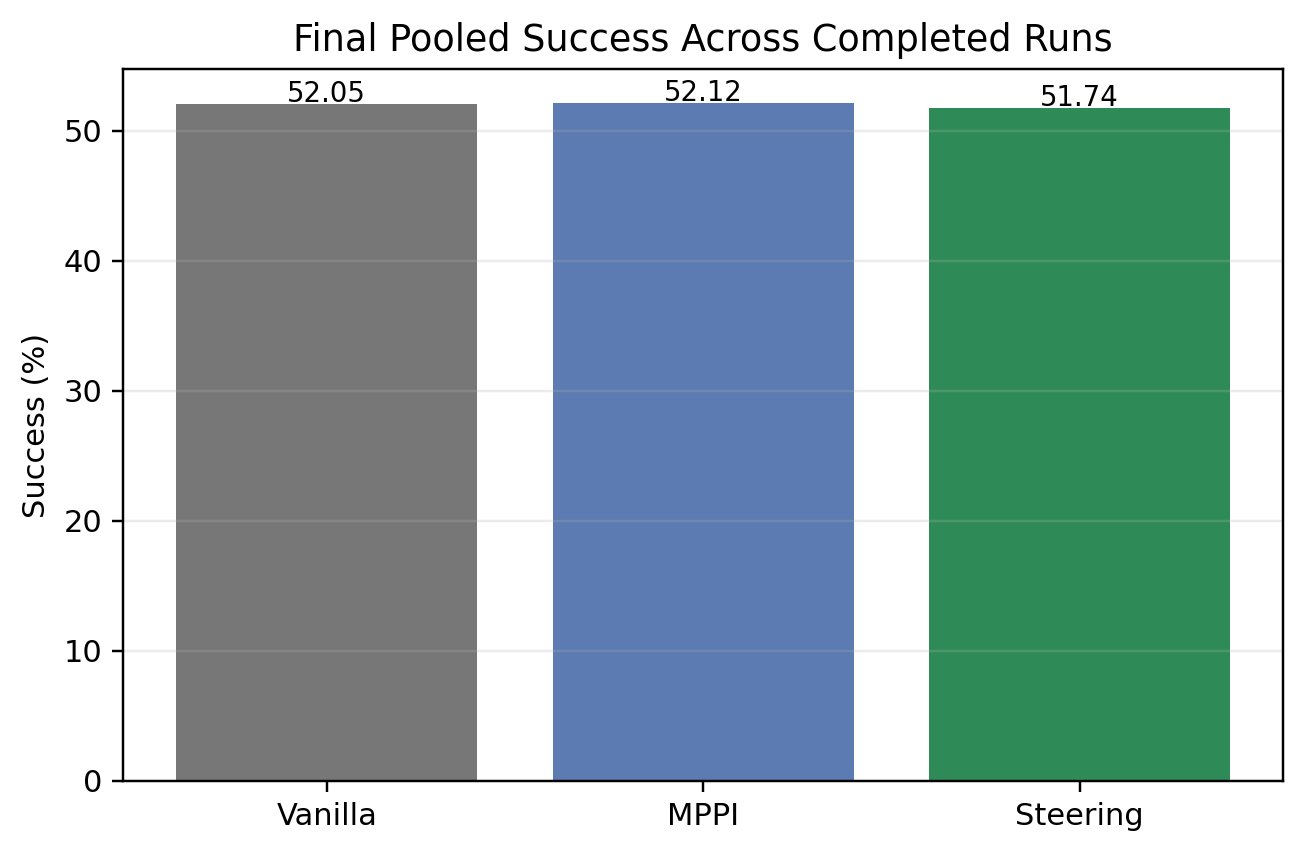
\includegraphics[width=\linewidth]{figures/10_final_pooled_success.png}
        \caption{Pooled success rates. Vanilla, MPPI, and single-step gating are TOST-equivalent (${\pm}2$\,pp); latent jiggle is the outlier (\S\ref{sec:mechanism}).}
        \label{fig:pooled_success}
    \end{subfigure}
    \caption{\textbf{Same success, $6.1{\times}$ lower latency.} The speedup is inference optimization: one probe query per step vs.\ $K{=}16$ on the same failure head, not a new task cost or certified safety layer.}
    \label{fig:latency_result}
\end{figure}

\begin{table}[t]
\centering
\small
\caption{\textbf{Pooled controller results} (OpenVLA + ACT, sweep + OOD + zero-shot). Success is binary task completion; 95\% Wilson CIs computed from raw episode counts. Apply time is mean per-step duration on the same A100 node across all pooled runs (warmup excluded). \textit{Latent Jiggle}: PULSE gating, random correction direction at matched magnitude---isolates the contribution of the correction head (\S\ref{sec:mechanism}). TOST equivalence (${\pm}2$\,pp) for all pairwise contrasts is in Appendix~\ref{app:stats}.}
\label{tab:final_pooled_results}
\setlength{\tabcolsep}{4pt}
\begin{tabular}{lcccc}
\toprule
\textbf{Method} & \textbf{Success (\%)} & \textbf{95\% CI} & $n$ & \textbf{Latency (ms)} \\
\midrule
Vanilla & 52.05 & [51.1, 53.0] & 10{,}000 & --- \\
K-sample MPPI & 52.12 & [51.1, 53.1] & 10{,}000 & 5.5 \\
\textbf{Single-step gating (ours)} & \textbf{51.74} & \textbf{[50.8, 52.7]} & \textbf{10{,}000} & \textbf{0.9} \\
Latent Jiggle & 52.90 & [51.9, 53.9] & 9{,}720 & --- \\
\midrule
Speedup (MPPI / ours) & \multicolumn{3}{c}{---} & $\mathbf{6.1{\times}}$ \\
$\Delta$(single-step $-$ MPPI) & $-0.38$\,pp & \multicolumn{3}{c}{TOST equiv.\ $p{=}0.011$~~$\checkmark$} \\
\bottomrule
\end{tabular}
\end{table}


Table~\ref{tab:final_pooled_results} reports pooled success across all completed runs ($n{=}10{,}000$ per mode for vanilla, MPPI, and single-step gating). All three primary pairwise $z$-tests are non-significant after Holm correction. TOST equivalence confirms statistical indistinguishability: vanilla ($52.05\%$) $\equiv$ K-sample MPPI ($52.12\%$) $\equiv$ single-step gating ($51.74\%$), all pairwise $p_{\mathrm{TOST}} \le 0.011$ at ${\pm}2$\,pp. Single-step gating achieves this at $0.9$\,ms vs.\ $5.6$\,ms per step ($6.1{\times}$ speedup, pooled over all runs; Appendix~\ref{app:latency_secondary} reports a benchmark-job crosscheck at $6.47{\times}$), enabling sub-millisecond safety decisions in closed-loop control (Fig.~\ref{fig:latency_result}). \textbf{The headline result is latency reduction, not success-rate lift}: all controllers sit at the base policy's ceiling on LIBERO-Spatial.

\subsection{Mechanism: Spatial--Control Decoupling}
\label{sec:mechanism}

To isolate what drives the latency result, we run \emph{latent jiggle}: the same MLP forward pass and magnitude gate as single-step gating, but the applied direction is a random unit vector at matched norm. Jiggle achieves $52.90\%$ pooled success vs.\ $51.74\%$ for learned steering; TOST equivalence at ${\pm}2$\,pp fails ($p_{\mathrm{TOST}}{=}0.119$; the small gap numerically favors jiggle). \textbf{Under time-matched labels on LIBERO-Spatial, temporal gating (when and how much to nudge) carries the closed-loop payload; learned spatial direction does not add a reliable success lift over random aim at the same magnitude.}

\paragraph{Spatial--control decoupling.}
Our finding that latent jiggle ties or numerically exceeds learned direction reveals a critical decoupling between offline ranking metrics and closed-loop episode success (\emph{spatial--control decoupling}). Strong offline directional scores (Table~\ref{tab:safety_head_metrics}) coexist with no reliable episode-level gain over jiggle (Table~\ref{tab:final_pooled_results}). This stems from three distinct system constraints:
\begin{enumerate}[leftmargin=1.4em, topsep=2pt, itemsep=2pt]
    \item[\textbf{(i) Scale mismatch.}] The probe tracks directional labels well offline (e.g., OpenVLA axis AUCs $0.85$/$0.88$/$0.78$), but the deployed controller clamps EEF adjustments to $\sim$3\,mm and rescales into action space---perturbations small enough that LIBERO's binary success predicate is largely insensitive to compass bearing.
    \item[\textbf{(ii) Shared magnitude gate.}] Jiggle is not a no-probe baseline: it preserves the MLP's predicted correction \emph{magnitude} and the same magnitude threshold. What is randomized is direction only. The operative bottleneck signal is therefore primarily \emph{temporal}---whether and how strongly to intervene---not the spatial vector returned by the correction head.
    \item[\textbf{(iii) Label vs.\ recovery.}] Targets $\Delta\mathbf{p}_t = \mathbf{p}^{\mathrm{succ}}_t - \mathbf{p}^{\mathrm{fail}}_t$ from time-index-matched nearest-neighbor trajectories optimize sequence matching, not recovery in an unfolding MDP. High offline AUC means the head learned the \emph{labeling convention}; it does not imply that label is an optimal closed-loop control direction.
\end{enumerate}
We caution against using offline spatial AUC or axis correlation as a proxy for deployable steering gain without closed-loop ablations on the target benchmark.

The decoupling is compatible with---not contradictory to---the directionality probe (Appendix~\ref{app:spatial_failure}): hidden states encode failure direction in the first $25\%$ of failure trajectories (displacement error $8.7{\to}7.6$\,cm on OpenVLA), but standard magnitude gating fires later, after proprioception catches up. The latent carries spatial information; under current labels and gating it is not translated into success lift. Recovery-conditioned demonstrations and earlier-firing thresholds (Appendix~\ref{app:threshold_sweep}) are the natural paths to re-couple spatial readout to control.

\subsection{Adaptive Gating and Generalization}
\label{sec:adaptive_gating}

\begin{figure}[t]
    \centering
    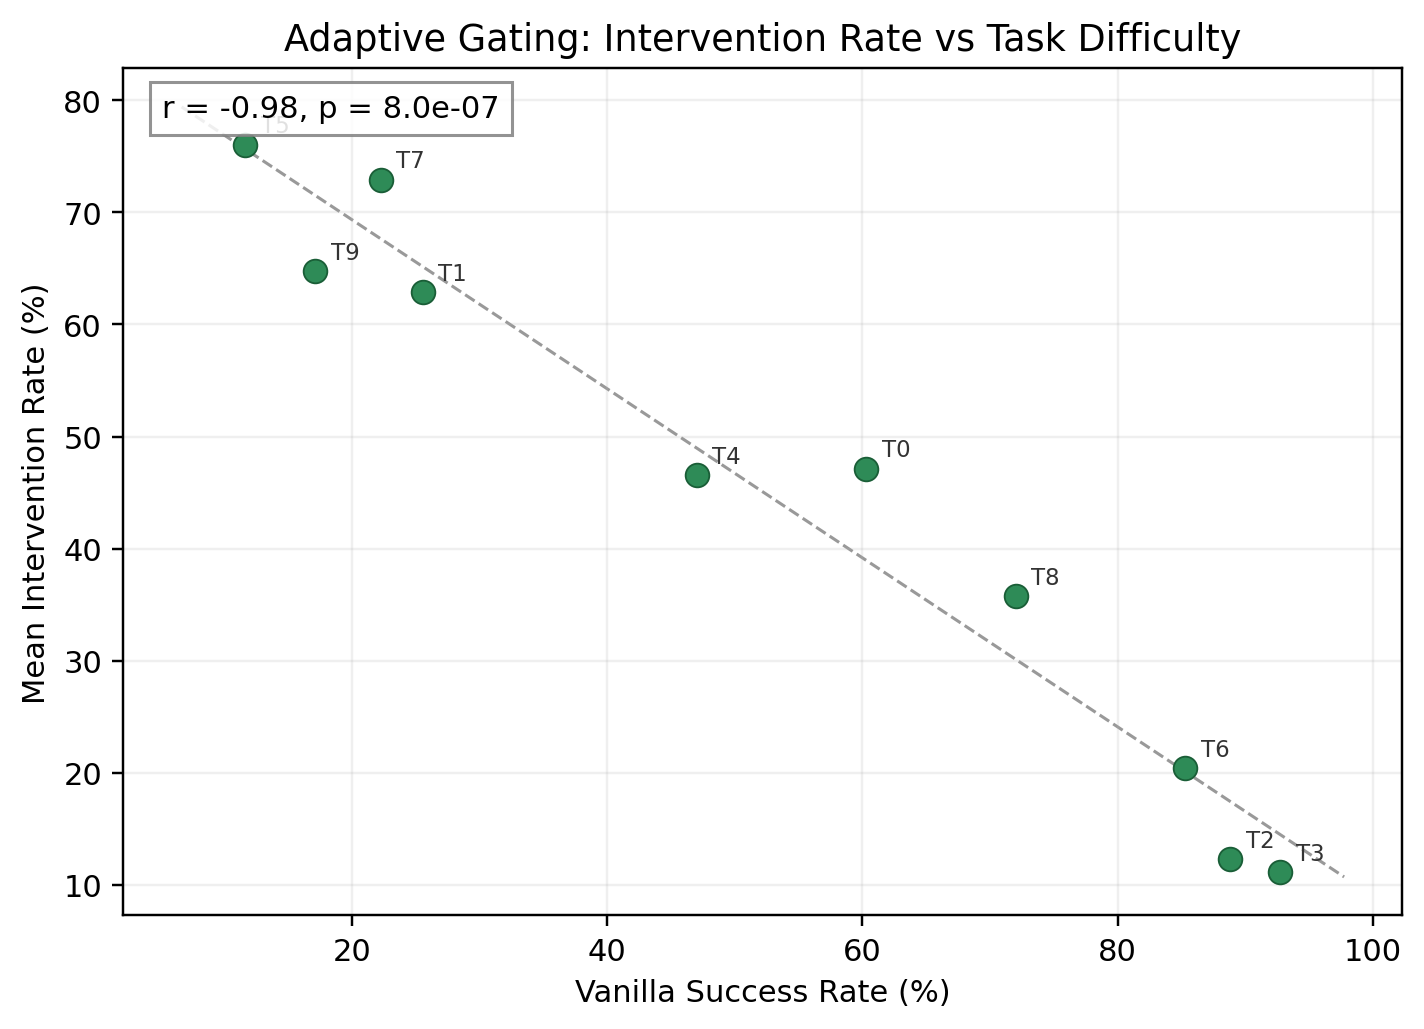
\includegraphics[width=0.65\linewidth]{figures/23_intervention_vs_difficulty.png}
    \caption{\textbf{Difficulty-responsive intervention.} Per-task intervention rate correlates at $r{=}{-}0.98$ ($p{<}10^{-6}$, $n{=}10$) with vanilla success---hard tasks receive dense intervention, easy tasks almost none, without any explicit difficulty signal.}
    \label{fig:intervention}
\end{figure}

\paragraph{Difficulty-responsive intervention.} Per-task intervention rate correlates at $r{=}{-}0.981$ ($p{=}5.2{\times}10^{-7}$; Spearman $\rho{=}{-}0.988$; $n{=}10$) with vanilla task success (Fig.~\ref{fig:intervention}). Pooled mean rate is $40\%$ of timesteps (median $37\%$; range $10$--$66\%$).

\paragraph{Zero-shot generalization.} Training on 8 tasks and evaluating on 2 held-out tasks with OOD push yields vanilla parity ($37.5\%$ vs.\ $38.2\%$, $p{=}0.86$): the probe does not hurt on unseen tasks.

\paragraph{Cross-architecture.} The same qualitative pattern holds on OpenVLA and ACT: vanilla, MPPI, and single-step gating stay within ${\sim}1$\,pp on each architecture (full table in Appendix~\ref{app:stats}). Linear cross-architecture transfer fails (ACT${\to}$OpenVLA AUC $0.27$; OpenVLA${\to}$ACT $0.42$)---the probe template is reusable but safety directions are architecture-specific and must be retrained per policy family.

\paragraph{OOD robustness.} Under $2$--$5{\times}$ baseline disturbance on the four hardest ACT tasks, the pooled single-step gating advantage ($+0.6$\,pp, $p{=}0.42$) is not significant. K-sample MPPI leads single-step gating by $3.0$\,pp on the hard ACT OOD sub-pool ($n{=}80$; not significant after Holm correction), suggesting MPPI's search advantage may emerge at extreme disturbance at the cost of $6{\times}$ latency---an engineering trade-off worth monitoring on harder benchmarks (Appendix~\ref{app:stats}).

\subsection{Physical Robot Evaluation}
\label{sec:physical_results}

{\color{blue}
Physical evaluation on SO-101 arms is in progress (protocol in \S\ref{sec:physical_protocol}). The primary metric is zero-shot failure-detection AUC on real hardware (target ${>}0.70$); secondary metrics are per-task success rate for vanilla vs.\ single-step gating ($N{=}50$\,ep/mode/task) and closed-loop latency on the embedded compute. Results will replace this placeholder for the camera-ready version.
}

